\section{Experiment - Identification of Garbage}
The first phase of the project was working on identifying garbage from an image. We tried to take an approach to train a Convolutional Neural Network to identify the garbage from an image and segment that part out. The first thing to do was to gather a large amount of labelled data (images of garbage) but before doing that we did our background research online to find any work done on this problem. Fortunately, we found a model already trained to identify garbage from the images. We decided to test that out and if that works, we could simply incorporate that model into our project.
\subsection{GarbNet Model}
The GarbNet Model was initialized on a pre-trained model, AlexNet, which is a model that is already trained on 1 million images of 1000-way object recognition. The architecture was customized to perform binary classification (is garbage, is not a garbage). More details about this model can be accessed by clicking on the heading $\-\>$ \href{https://dl.acm.org/doi/pdf/10.1145/2971648.2971731}{GarbNet Model - SpotGarbage}.
\section{Experiment - Quantification}
In this project, we tried different approaches for quantifying the volume of the garbage from an image. Those approaches are described in detail in the Literature Review (\ref{chap:lit}) section of the report. This section will briefly talk about all the methods, along with their advantages and disadvantages.
\subsection{3D Reconstruction from Multiple 2D Images}
This approach uses 2D images taken from different angles to reconstruct a 3D image. Susheel [5] proves that using 2D images from 8 different angles would improve the accuracy of our model to about 85 percent. This method seemed promising but given our target audience, the common man, this seemed a bit unrealistic. We came to the conclusion that not a lot of people would go around taking 8 different pictures of the same garbage dump from 8 different angles and therefore, we dropped this methodology and tried our luck with Depth Analysis and Stereoscopic Vision methodology.
\subsection{Depth Analysis and Stereoscopic Vision}
This approach uses two camera lenses spaced slightly apart to let the phone compare two images and piece together the depth of the object in stereo. With this methodology, using two cameras and their features, the accuracy of the model was promising (in theory) but we could not take this idea to its implementation because if we were to use this methodology in our project, then it would become a pre-requisite for the user of our app to have two cameras at their disposal, which was quite unrealistic. Therefore, we dropped this methodology and tried our luck with Dimension of Object - By Reference methodology. 
\subsection{Dimension of Object - (By Reference)}
This approach uses the camera parameters (DPI, Focal Length, etc.) of the device along with a reference object in the image with a known width and length. We tried this method, implemented it with our project and it was giving a very good result. However, one drawback of this method was that for every picture of the garbage dump that the user will upload on the app, they need to have a reference object (a human, a table, a chair, etc.) with a known width and height. Keeping in mind our target audience, the common man, this seemed unrealistic that all the images will have a reference object. Therefore, we dropped this methodology and tried our luck with Dimension of Object - By Distance methodology.
\subsection{Dimension of Object - (By Distance)}
The fundamental idea behind this approach is to still find the dimension of the object (garbage dump) from the image and using those dimensions, we can easily calculate the volume of the object. To get the dimensions of the object, we need to know the actual width and height of the object. We can get width if we have the height and vice versa. The methodology implemented uses camera parameters, the distance of the object from the camera (an approximate distance of the user from the garbage). 
\begin{figure}
    \centering
    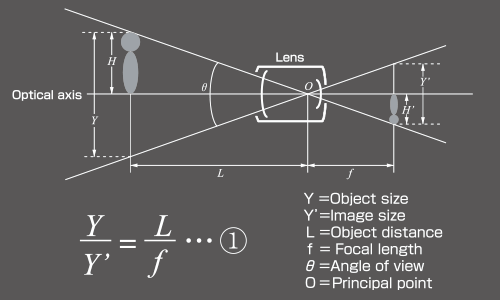
\includegraphics[scale=0.6]{images/dimensionDistance.png}
    \caption{Proportional Ratio of lens}
    \label{fig:lensRatio}
\end{figure}
\\
The equations used are as follows:
\begin{equation}
    \frac{Object Dimension}{Distance} = \frac{Object on Sensor Dimension}{Focal Length} 
\end{equation}
\begin{equation}
    Object Height = \frac{Object on Sensor Height * Distance}{Focal Length}
\end{equation}
where Object Height (m) - value to find,\\
Object on Sensor Height (mm) - get this in terms of pixels,\\
Distance (m) - User will input this hyperparameter,\\
and Focal Length (mm) - can be obtained by camera.\\
As mentioned above, we already are getting focal length and distance and we can simply put in the values in the equation and get the result. One drawback of this approach was that, we could only extract height from image in terms of pixels. We needed the height on sensor in terms of mm (the actual distance). One method that we tried was converting pixels into mm via dots per inch/ pixels per inch.  We need height in terms of \textbf{mm} and we are getting in terms of \textbf{pixels}. The equation below will show you the reasoning and mathematics behind it. 
\begin{equation}
    1 Pixel = \frac{25.5 mm}{Dots/Pixel Per Inch}
\end{equation}
How many pixels are on 1 inch of screen? We can get that using the equation below:
\begin{equation}
    Dots/Pixels per Inch = \frac{Pixel Diagonal}{Screen Diagonal}
\end{equation}
where as we can get xdpi and ydpi from the android application, and height and width in pixels, and height and width of phone screen.\\
However, the resulting height of the garbage in terms of mm was being incorrectly calculated using this methodology. The reason was that we were calculating in terms of dots per inch but that was also dependent on sensor of the camera. So we needed to focus on getting the the dimensions of sensor. Only then can we effectively convert the image from pixels to mm. Therefore, we had to stop using dpi/ppi and find another method to convert from pixels to mm. One method we tried was using Field of View of the lens. It was the angle at which our camera works. The below figure will give you an idea of how it is used:\\
\begin{figure}
    \centering
    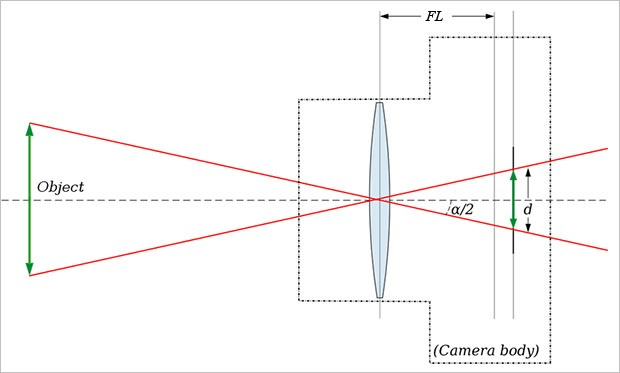
\includegraphics[scale=0.5]{images/fov.jpeg}
    \caption{FOV relation to the Image}
    \label{fig:fov}
\end{figure}
\\
Using the properties of ratios, we can tell that through the camera angle (Field of View), the image is projected on to the sensor. Using this information and trigonometry, we can get the width and height of the garbage using either horizontal angle or vertical angle. The equation, in either case, would be as follows:
\begin{equation}
    Sensor Width = tan(horizontal angle/2) * 2 * Focal Length   
\end{equation}
Once we have the sensor width, we can simply calculate the width of garbage in mm using the following equation:
\begin{equation}
    Width of Garbage (mm) = \frac{Width of Garbage in Pixels * Sensor Width}{Width of Entire Image}
\end{equation}
Once we get the width using the horizontal angle, we can then simply use the ratios between the original width and pixel width to find the original height of the garbage using the following equation:
\begin{equation}
    Original Height (mm) = \frac{Original Width * Sensor Height}{Sensor Width}
\end{equation}
Now, once we have the height and width of the garbage from two different images, we can then use them to find the volume of the garbage.
\section{Optimizations}
Once we had the volume, we realised that the volume is a bit of an overestimate of the actual volume of the object. This was due to the fact that spotgarbage (the GarbNet model) always produces an overestimate bounding box of the garbage dump. Taking that into account, we tried to find ways to reduce that effect of overestimating and in return, optimizing our model. One method that we tried was that we tried multiple objects with known bounding boxes and compared them with the output of the spotgarbage. This way, we found an average percentage error that the GarbNet model was making and how much it was overestimating. Using the findings from this experiment, we put an underestimating multiplying factor to the final bounding box and found that it gave much better results than the previous implementation. Once we got the bounding boxes of our object (garbage patch) at hand, we calculate the volume of those bounding boxes within which our garbage is encapsulated. We use known volumes of regular shapes to better our calculation results of the irregular shapes. We use the shape of the pyramid and cube with its known volume to make a sense of how  our final calculated volume could come as close to the actual volume of our irregular shaped garbage.
\section{Result}
The resulting product of our project is an Android Mobile Application that communicates with the Web Admin Portal through third party Cloud Storage and Services.
\subsection{Android Mobile Application}
The application was developed on Android Studio that uses java as its back-end language, and xml as its front-end and linking language. The implementation and design of the Android Mobile Application is displayed in the SDS section (\ref{chap:sds}) above.
\subsection{Cloud Storage and Services}
Early on in the development stage, we focused on Amazon Web Services platform for our cloud related queries. At the same time, we also explored Google Cloud Platform as a backup plan in case AWS doesn't work out. Comparing those two platforms and its user interface and friendliness, we switched to Google Cloud Platform because it was much more easier to understand and navigate. More information about this can be found in the SDS section (\ref{chap:sds}) above.
\subsection{Database - Google Firebase}
As mentioned above, we decided on using Google Cloud Platform and thus used Google's mobile application development platform (Firebase) as our real time database for the project.
\subsection{Web Admin Portal}
Web Admin portal was developed using website development tools (html, javascript, css, etc.). It's a portal that uses the Google Cloud Platform to communicate with the mobile application.  More information about this can be found in the SDS section (\ref{chap:sds}) above.

\subsection{Integration}
As mentioned above, we had three stand alone resulting products of our project: Mobile App, Cloud Model, Web App. Integration deals with integrating the three stand alone parts into one complete final product known as Project Cleanup. \\
\\
The way we integrated that was that we developed a python script that listens onto the bucket in the Firebase Real Time Database and whenever a new job is posted from the mobile app, the listener gets triggered and the script starts executing. The basic overflow of the script is as follows: The job posted has some images with it that are stored in firebase. The script downloads those images from firebase to its base location on Google Cloud Storage and passes it through the GarbNet model to segment out the garbage in the image.\\
\\
Once GarbNet recognizes the garbage, the segmented part is then passed onto the Quantification model that calculates the volume of the garbage in the images and update the volume's value back on the firebase, which can later be accessed by the Web Admin App to display the information about each job, their location, and the approximate volume of garbage present there.\\
\\
There were some challenges that we faced along the way. One challenge was integrating firebase with javascript, it was very difficult to do that but in the end, it got resolved. Another challenge was making the flow of the final product as smooth as possible with minimum delay in between.\\
\\
Having said all that, the project is fully functional with the Mobile App, Web App and the Cloud Script ready. The script hosted on Google Cloud runs 24/7 and listens for job posting through the mobile app.